% Chapter 8

\chapter[Application Design]{Application Design} % Main chapter title

\label{Chapter8} % For referencing the chapter elsewhere, use \ref{Chapter8} 

%----------------------------------------------------------------------------------------

\section{Overview}
This section describes the design of the application, and gives details on the reasoning behind some of the design decisions. This design work was done largely prior to implementation, with some elements of the design being re-factored during the implementation phase in adherence to the agile development methodology being followed. The design process was broken down into two key areas. Firstly the design of the software architecture, including the breakdown of the different components and the path of data through the system. This served as a road map during the implementation stage. The second key design area was the user interface. This involved sketching out the window layout and deciding how best to provide the user with access to the various features.

%----------------------------------------------------------------------------------------

\section{Software Architecture Design}
The guiding principles of the software architecture design were the ideas of `Object Oriented Programming' (OOP), and the `model-view-controller' (MVC) software architecture pattern. OOP [OOP REFERENCE] is an extremely widespread concept in software development theory. The basic idea is that code should be organised into units based on individual functionalities, commonly referred to as classes, where the data that describes an object and the routines to perform actions with and on that data are collected together. An object usually refers to a single instance of a class. OOP aims to reduce duplication in code, make code easier to understanding and maintain, and increase re-usability and modularity. Designing software in an OOP fashion is standard practice for most modern programming tasks, and modern languages are often designed around OOP concepts. C++ was selected as the development language for this application for several reasons. The majority of the existing software infrastructure in the YRL has been implemented in C++, hence following suit would help with maintainability in the future. C++ also offers much of the low level control and efficiency of the C language, whilst also supporting OOP practices natively. Considering the project's requirements for interfacing with low level hardware such as the tracking camera via the camera drivers and the robots via network sockets, and for performing image processing, the speed and low level capabilities of C++ seemed beneficial. Higher level languages such as Java were considered, as they offered a number of different benefits such as better portability and resource management, but this was ultimately deemed less valuable.

The MVC software architecture design pattern is another widespread concept in software development theory. It primarily relates to the programming of application user interfaces. The three words that give the pattern its name define the three 'layers' into which code components are organised. The model refers to the application's data, and includes all of the information that defines the application in its current state. The view refers to the code used to produce the user interface from the data in the model. It acts as the method by which the user 'views' the data, thus getting its name. Finally the controller layer acts as the intermediary between the two, retrieving data from the model and processing it if necessary before passing it to the view for display. The controller also responds to data input events and changes the model accordingly. This includes data input via the user through the view, as well as data from other sources. In the case of this application these other sources include peripherals, such as the tracking camera, and the robots via the WiFi network. Adhering to an MVC pattern helps to keep code structured and organised, making it easier to understand, maintain and extend. It ensures that state data is not maintained by the UI, and that one true `gold standard' version of the application data exists within the model. 

With these two principles in mind, the software design process could begin. First the application was broken down into individual components based on the functionalities expressed in the functional specification. The following key areas were identified:

\begin{itemize}
\item Code relating to communicating with the camera
\item Code relating to performing the robot tracking
\item Code relating to handling networking and receiving data from the robots
\item Code relating to storing the robot data
\item Code relating to augmenting the video feed based on the stored data
\item Code relating to displaying the video feed to the user
\item Code relating to other elements of the user interface
\item Code relating to storing user settings
\item Code relating to producing logs of the data and events
\end{itemize}

Once separated into functional components, these components could be organised into a structure, and the data path of the application examined. Figure \ref{fig:SoftwareArchitecture} shows this structural arrangement, with boxes for each of the functional objects and arrows indicating data flow. The three layers of the MVC design pattern are shown by the vertical partitioning. The horizontal partitioning is used to show another key design consideration - threading. In order to maximise performance and ensure responsiveness, functionality which has the potential to `block' execution whilst waiting for a result or response should be run in a separate thread. This application was therefore designed with three threads in mind. The main thread handles the core of the application, including all data model access and GUI operations. The network thread handles communicating with the robots via WiFi. It was anticipated that this networking would involve low level socket code, which meant the potential for blocking socket-read operations, therefore requiring a separate thread. The camera thread handles reading the machine vision camera and performing the tag tracking using the ARuCo library. It was anticipated that the camera read operation could block until the next frame was available in the camera driver's buffer. Tracking the robots in the image using the ARuCo library also had the potential to be CPU intensive, so keeping this off the main thread was considered a potential performance benefit.

\begin{figure}
	\centering
	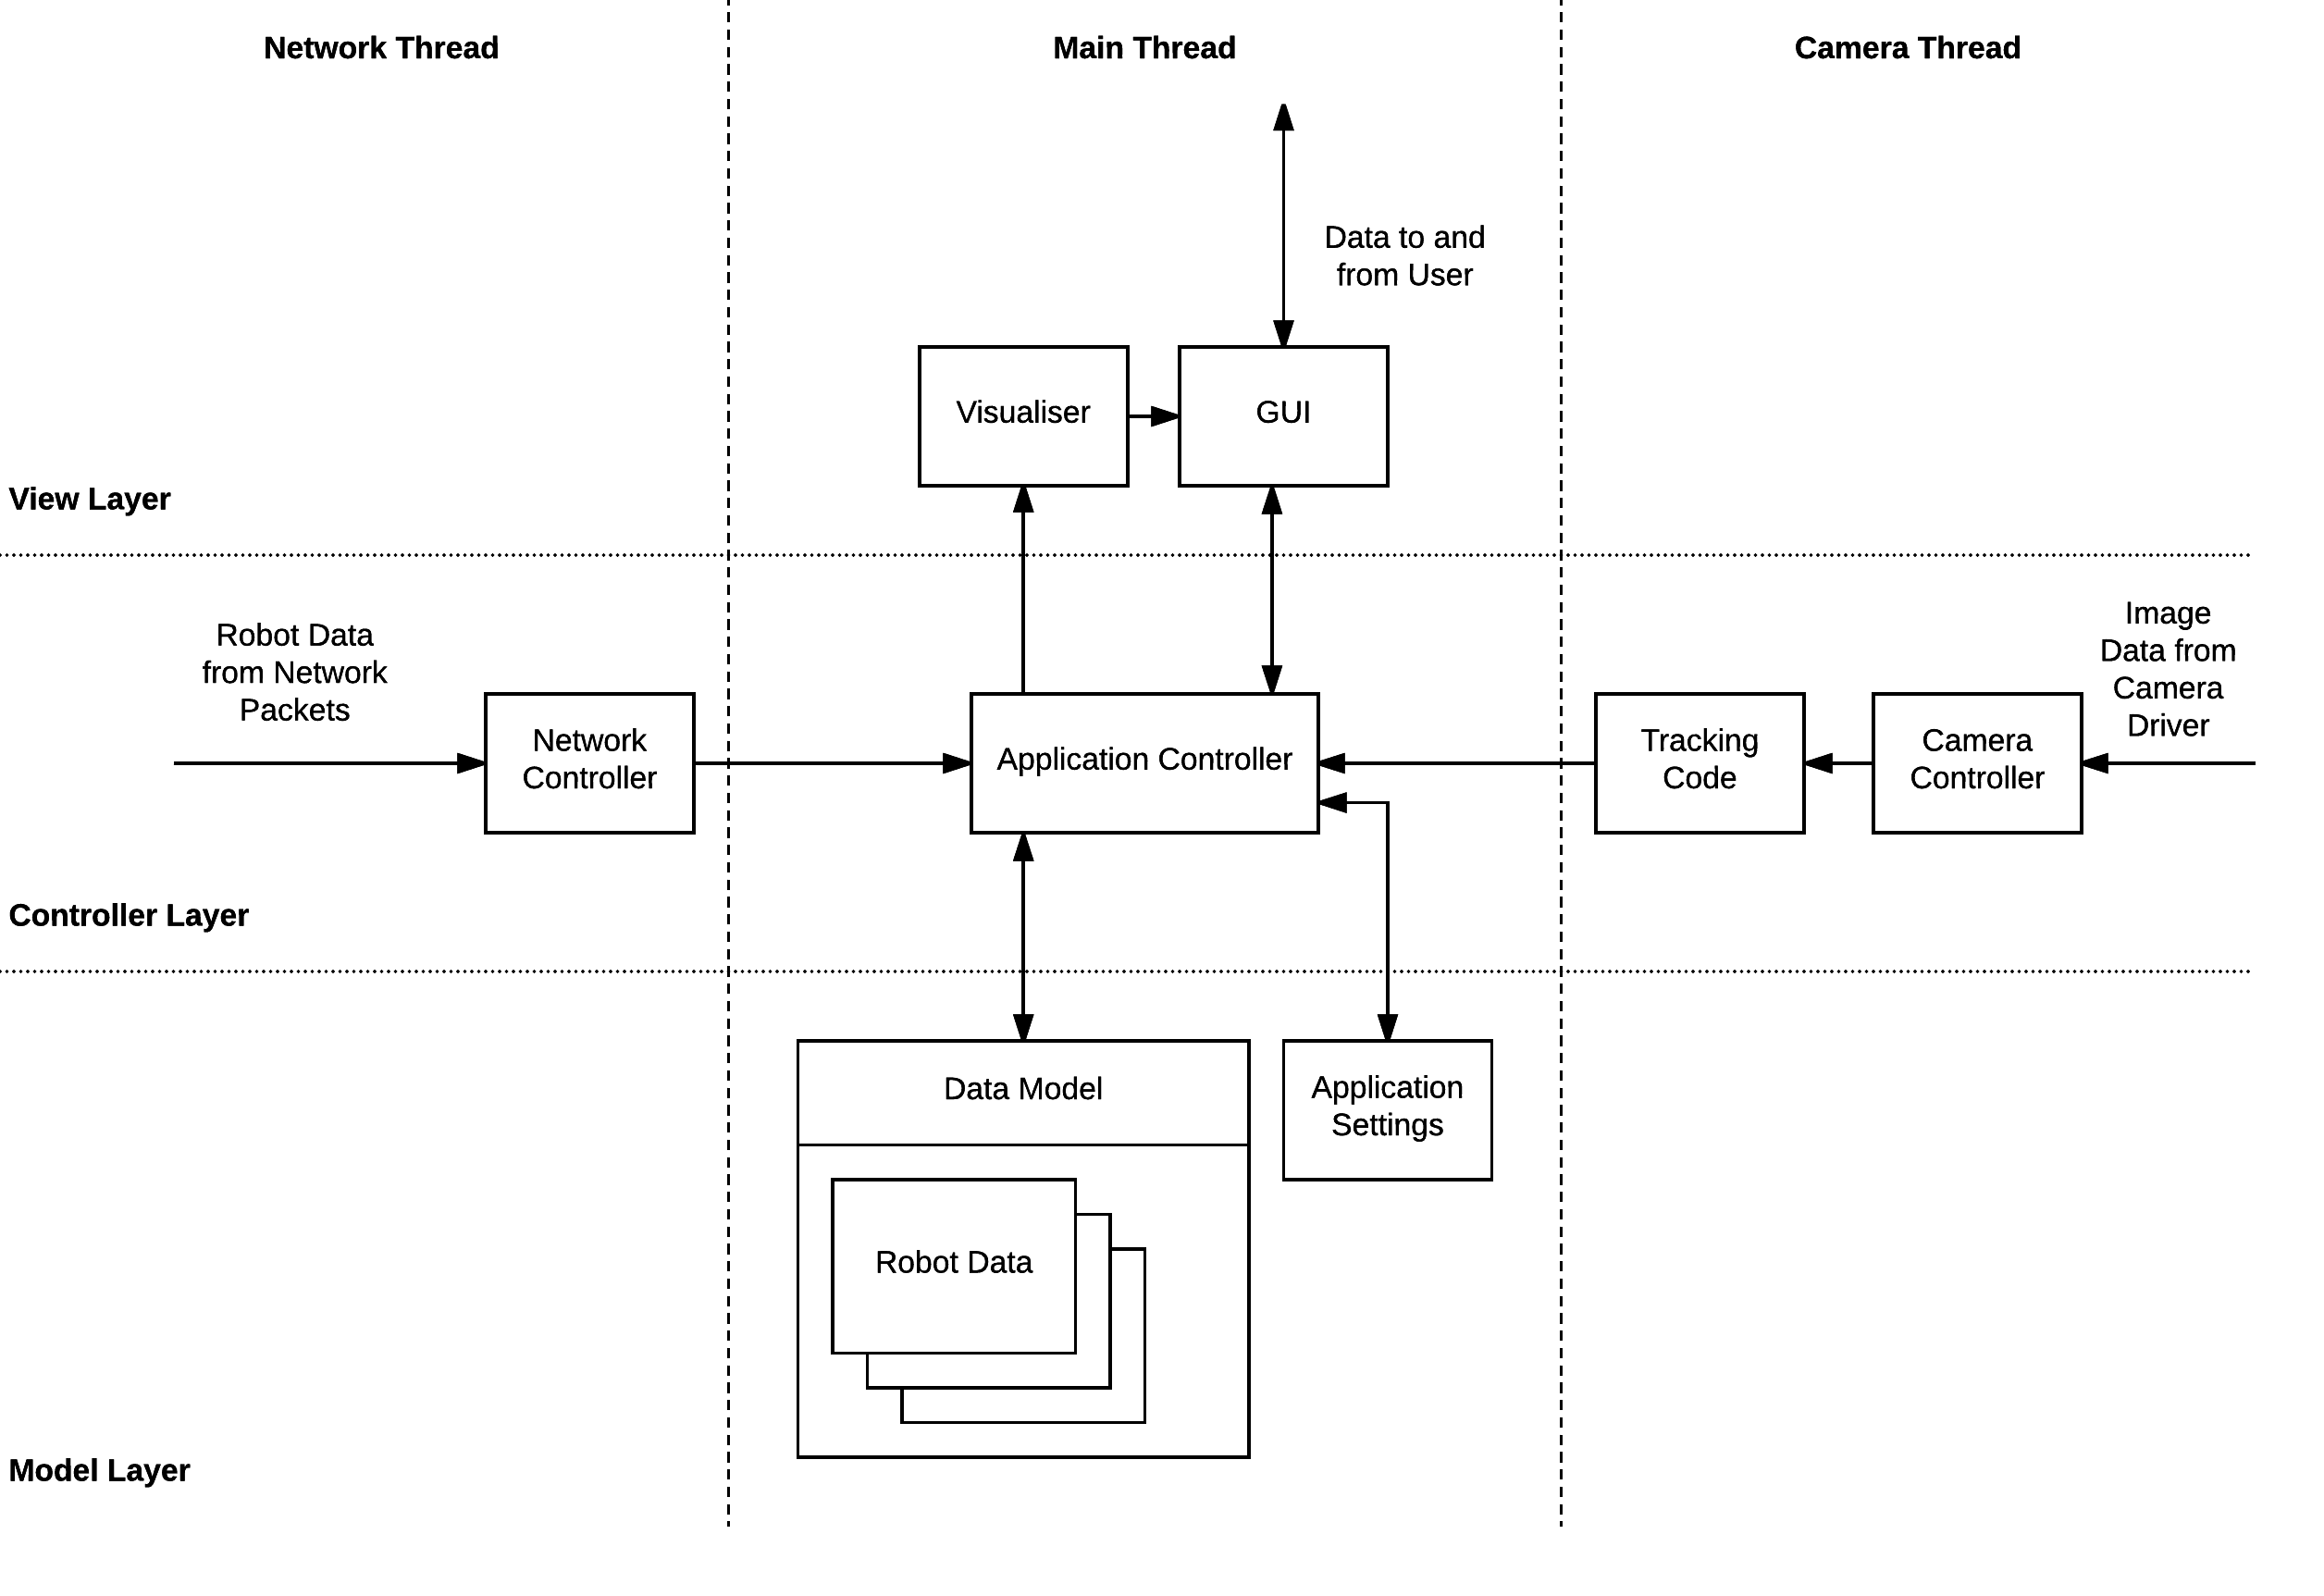
\includegraphics[scale=0.7]{Figures/SoftwareArchitecture.png}
	\decoRule
	\caption[Software Architecture Diagram]{A diagram of the software architecture design and data flow.}
	\label{fig:SoftwareArchitecture}
\end{figure}

\subsection{Data Model}
Figure \ref{fig:SoftwareArchitecture} also shows that the model layer contains the application settings and the data model. The data model itself was designed to be comprised of a number of smaller components. The primary function of the data model is to maintain a record of all the robots the system is aware of, and the most up to date data related to the state of each robot. As such the data model was designed to use a hierarchical structure. The larger data model object would maintain a collection of smaller objects, each containing the data related to a single robot. These would in turn maintain a collection of different data objects relating to the robot's state and sensor data. Figure \ref{fig:DataModel} illustrates this hierarchical data model design using the IR sensor data of a single robot as an example.

\begin{figure}
	\centering
	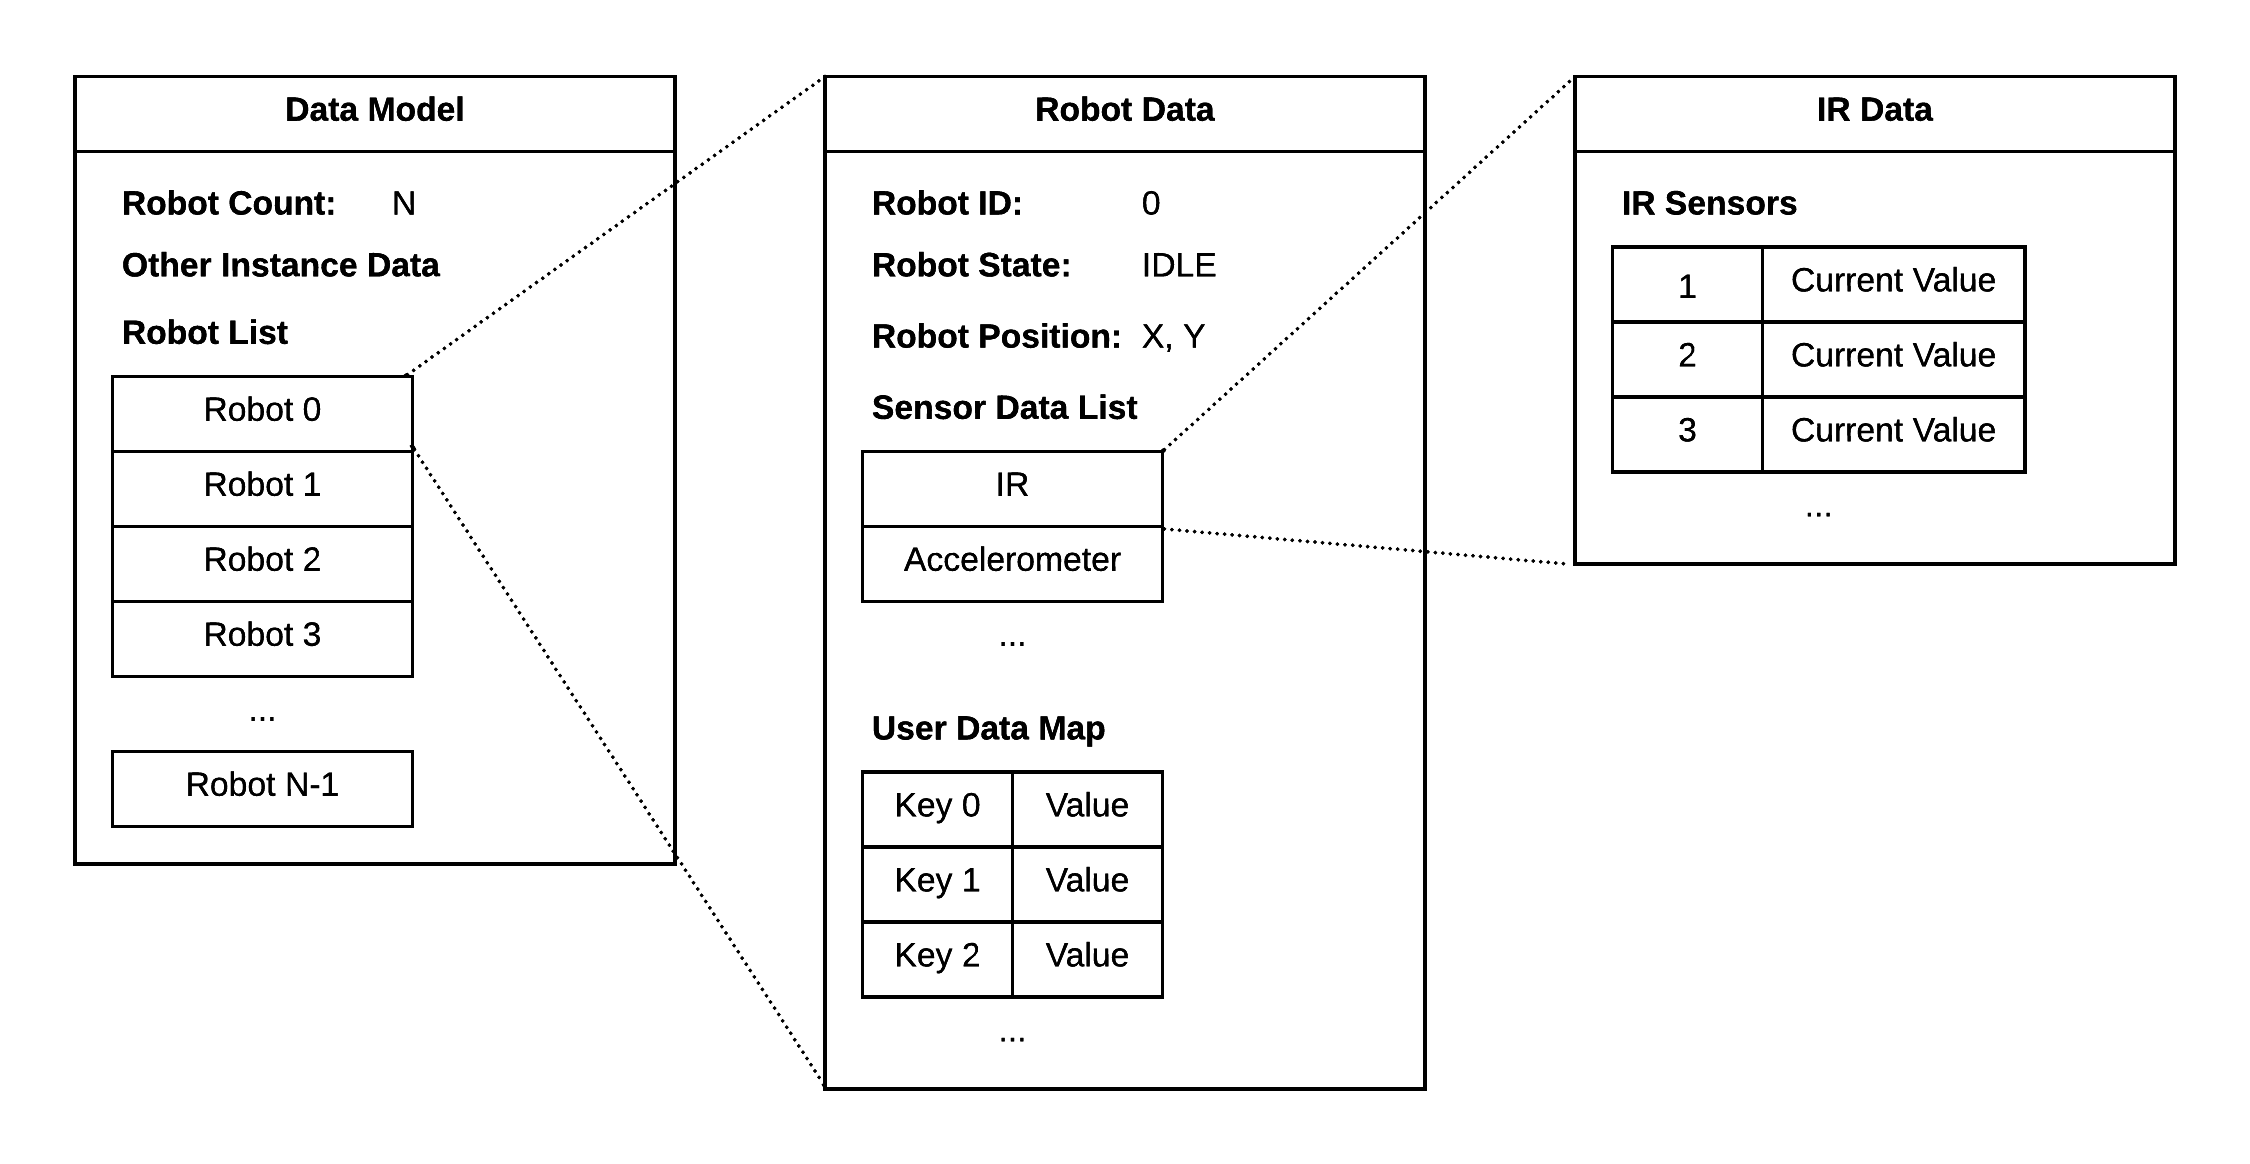
\includegraphics[scale=0.7]{Figures/DataModel.png}
	\decoRule
	\caption[Data Model Diagram]{A diagram of the data model design.}
	\label{fig:DataModel}
\end{figure}

%----------------------------------------------------------------------------------------

\section{User Interface Design}
The second main area of consideration during the design phase was the Graphical User Interface (GUI). It was determined that a well designed, intuitive interface would be essential to satisfying the objective of providing the user with data in a 'human readable' form, in real time. Having real time data would be useless if the user cannot also parse the data displayed in approximately real time. The first decision made was to try and keep the interface familiar to a computer user, through the use of standard, widely understood user interface elements. There exists a well defined `language' in computer interface design, using constructs such as windows, tabs, buttons, text fields and other elements which have well understood functions. It was thought that basing the user interface design on this well established standard would minimize the time for a new user to become accustomed to the system. The next step was determining how many windows would be necessary for the intended functionality to be possible, and how best to lay these out and organise the other elements within each. Three main windows were determined to be necessary. The first would display the video feed and visual overlay, the key component of the application. A second window would be used to display a list of the robots known to the system, so that they could be selected without obscuring the visualiser. Finally a third window would be used to display more detailed information about the selected robot in a number of different tabs. Figure \ref{fig:UILayout} shows the basic layout decided on for these three windows.

\begin{figure}
	\centering
	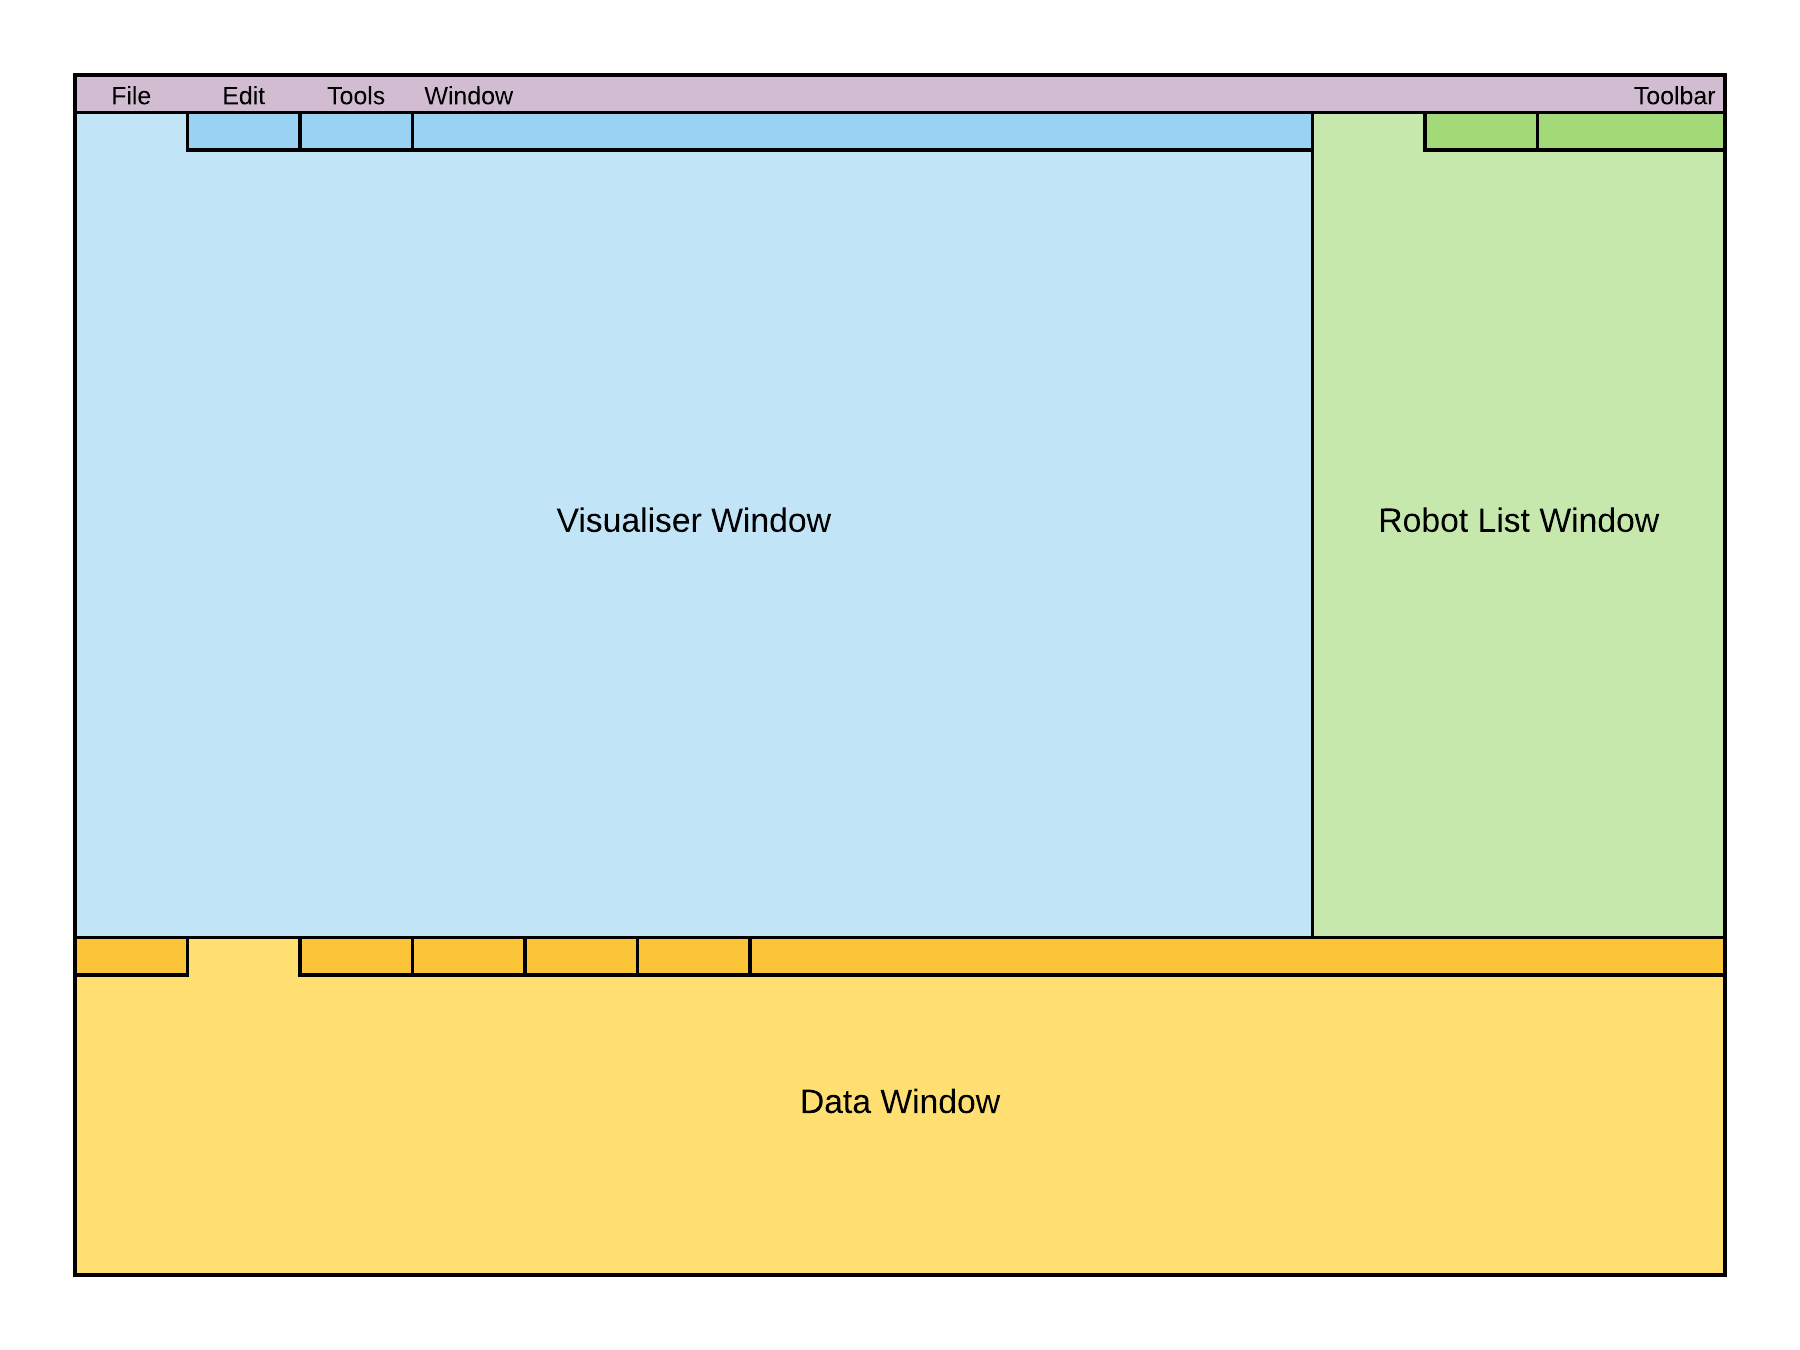
\includegraphics[scale=1]{Figures/UILayout.png}
	\decoRule
	\caption[UI Layout]{The design of the basic user interface layout.}
	\label{fig:UILayout}
\end{figure}

The visualiser window, highlighted in blue, takes primary place in the layout. In order to maximise the readability of the augmented video feed it was determined that this window should occupy as much space as possible. A number of tabs would then be contained in this window to give access to various settings, including settings for the visualiser. The robot list window is highlighted in green on the right hand side. This window requires less width, as it's main function is simply to display the robot list. A number of tabs would also be added here, to allow access to functionality related to the robots such as settings for the network connection. Finally the data window is highlighted in yellow at the bottom of the layout. The tabs would be used to provide more detailed info on each type of data collected about the selected robot, as well as a tab for a general overview, and a console-style log of application events. It was noted that when displaying data in this window it should be formatted to maximise the use of the available space. This means using the full width of the window and limiting the height to avoid scrolling. The design also includes a toolbar at the top of the window, another standard feature of window-based software applications.

\subsection{The Qt Framework}
In order to make creating this interface feasible, a GUI framework needed to be selected. Many GUI frameworks exist, each with various benefits. For this application the Qt Application User Interface framework for desktop was selected. This framework provides a comprehensive library of classes and an application programming interface (API) for implementing desktop user interfaces, with support for all the standard features of window-based applications. The Qt framework was chosen for a number of reasons. The framework is fairly widely used, and therefore has a well-tested, refined, and mature API, with a good body of documentation available. Previous experience with Qt outside of this project had been positive, and meant a smaller learning curve would be necessary to get started developing with it. For non-commercial projects Qt is also available free of charge, making it a good fit for an academic project such as this.

%----------------------------------------------------------------------------------------